%%%% this figure MUT BE READ BEFORE we can reference it in the text!!!!
\begin{figure*}[t!]
\vspace*{-4ex}
\centering
%\setlength{\tabcolsep}{3pt} % Default value: 6pt
%\renewcommand{\arraystretch}{0.5} % Default value: 1
%
%\begin{tabular}{lll}
%
%\begin{tabular}{c} 
%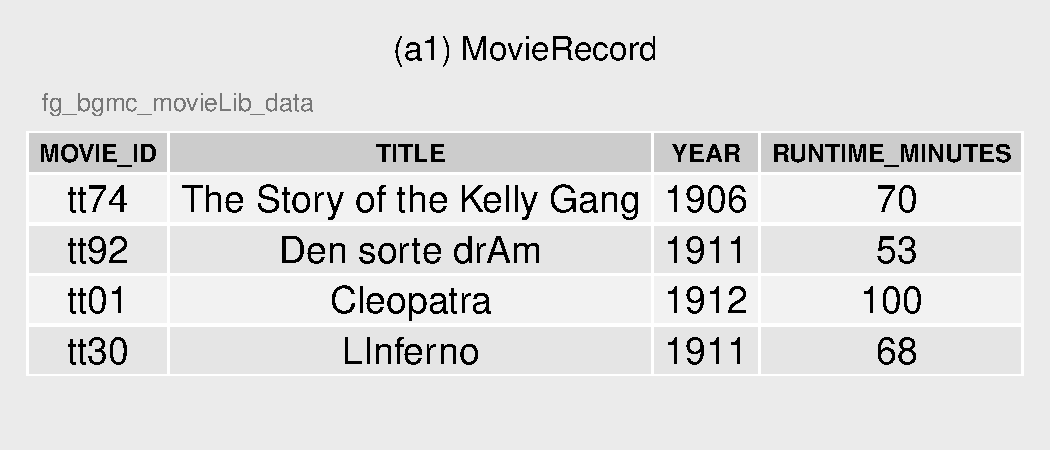
\includegraphics[width=0.33\textwidth]{../_Figures/fg_bgmc/fg_bgmc_movieLib_data_a1} \\
%\\[1ex]
%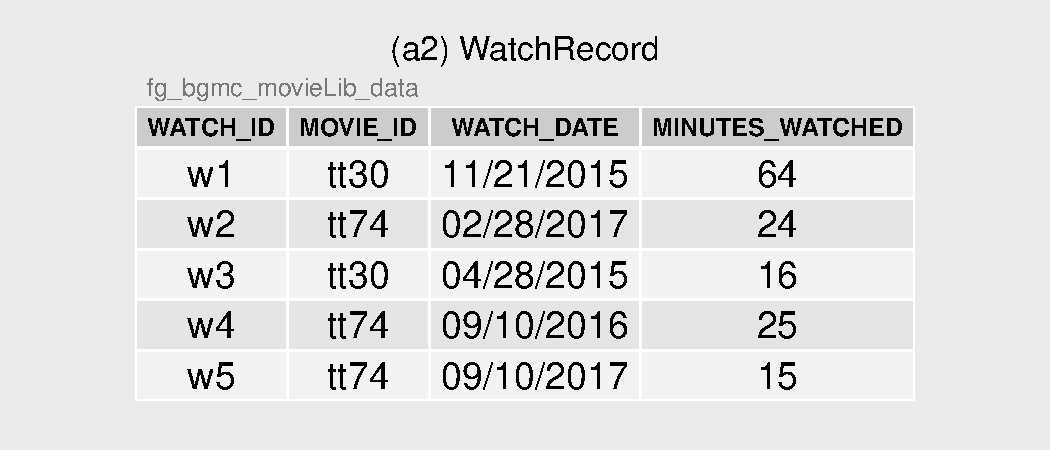
\includegraphics[width=0.33\textwidth]{../_Figures/fg_bgmc/fg_bgmc_movieLib_data_a2} \\
%\end{tabular} 
%
%&
%
%\begin{tabular}{c} 
%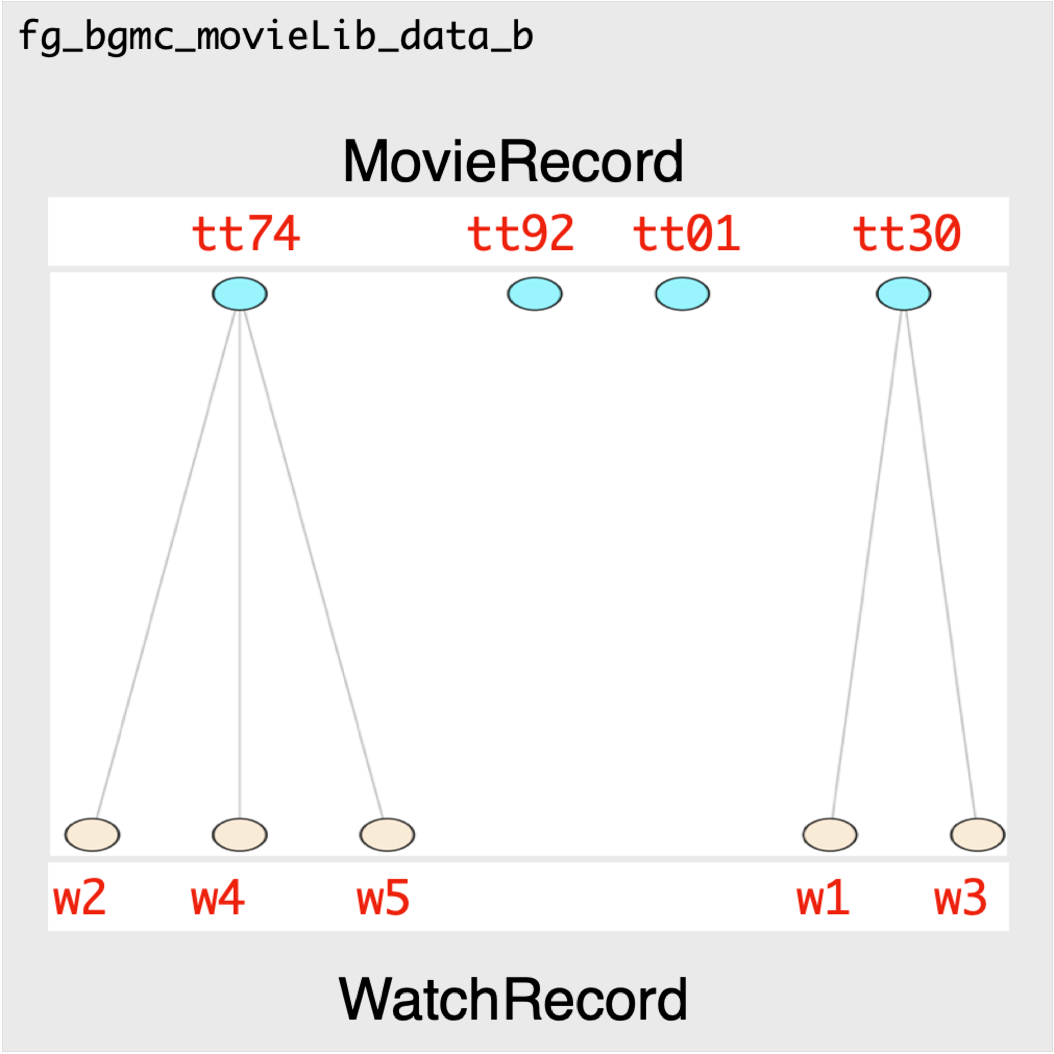
\includegraphics[width=0.31\textwidth]{../_Figures/fg_bgmc/fg_bgmc_movieLib_data_b}
%\end{tabular}
%
%&
%
%\begin{tabular}{c} 
%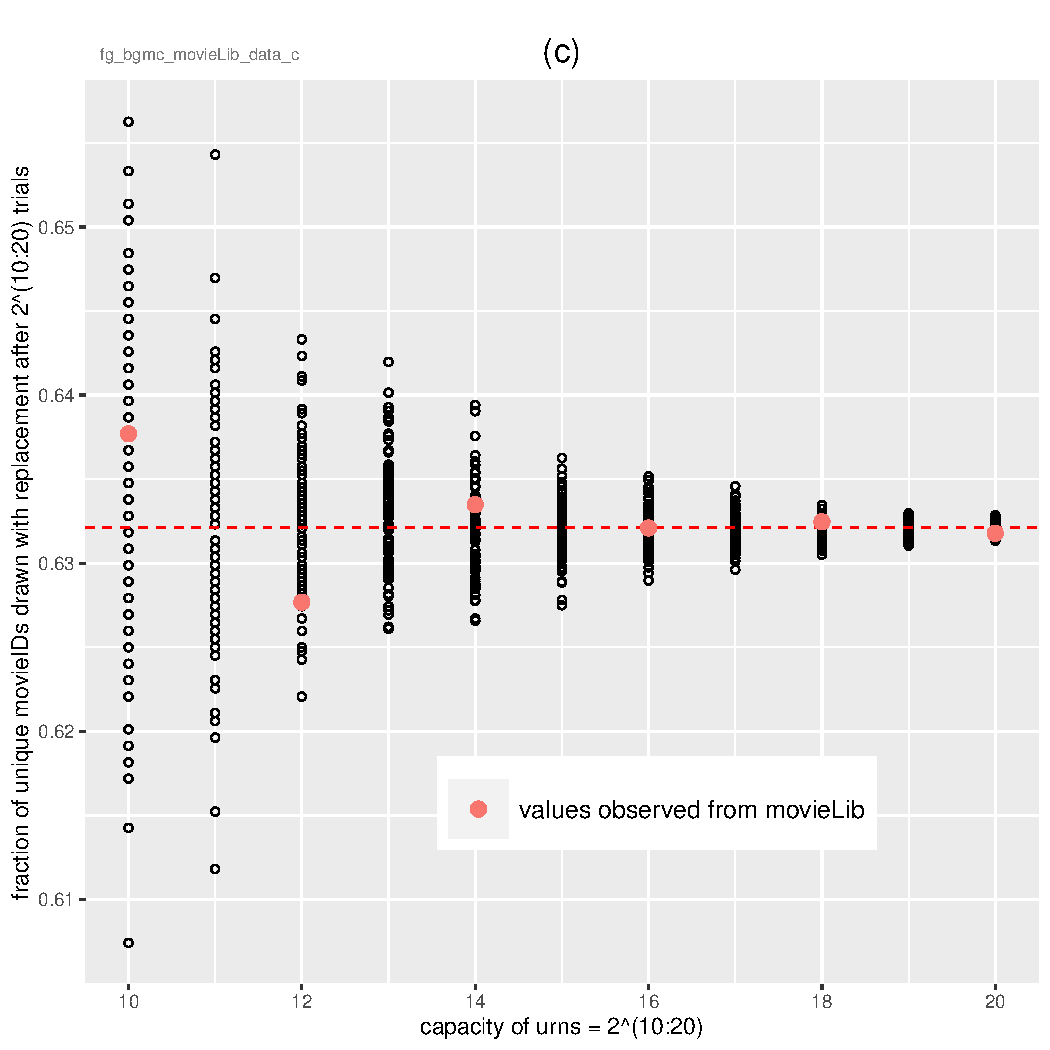
\includegraphics[width=0.33\textwidth]{../_Figures/fg_bgmc/fg_bgmc_movieLib_data_c}
%\end{tabular}
%
%\end{tabular} 

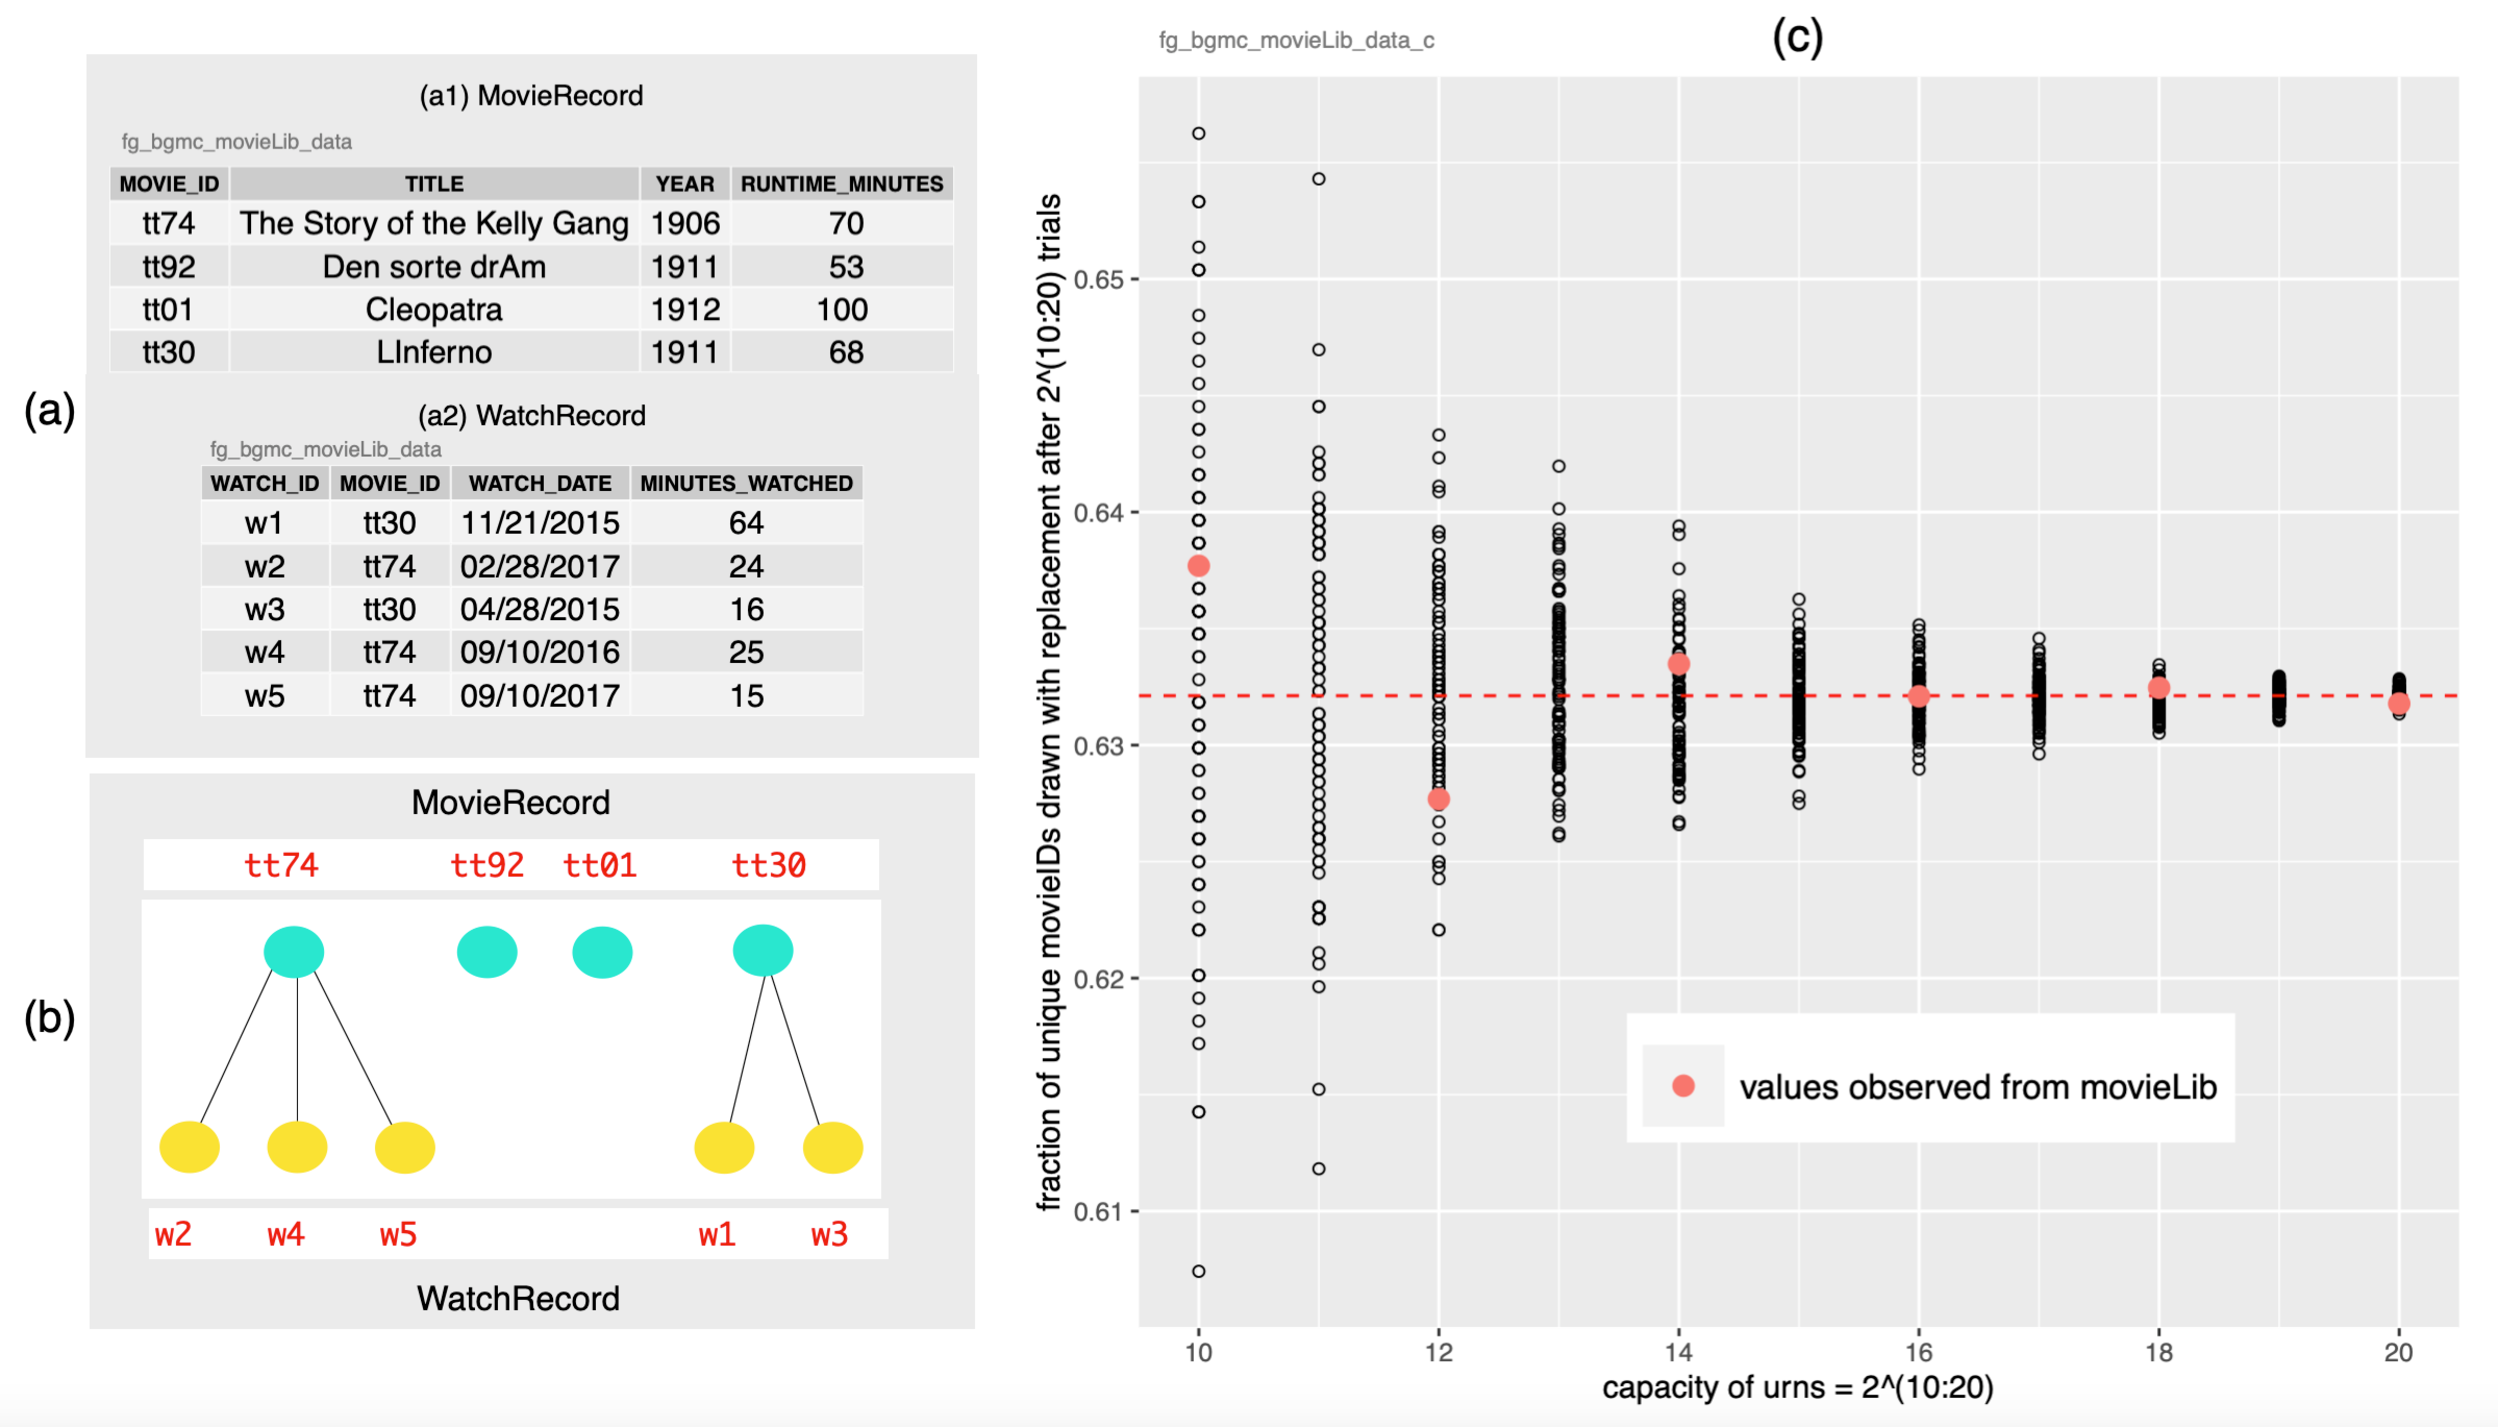
\includegraphics[width=1.00\textwidth]{_Figures/fg_bgmc_movieLib_data_abc}

\caption{Representations of data sets used in the performance experiments with 
the {\it MovieLib}   
data set introduced in Section~\ref{sec_316}:
{\sf (a)}~a tabular organization of files {\it MovieRecord} and  {\it WatchRecord}, 
{\sf (b)}~a bigraph that illustrates relationships between the
items from the two files in (a), and
{\sf (c)}~a statistical model, based on $2^{10}~...~2^{20}$ trials of sampling with replacement   
from 11 urns, each with urn capacity of holding $2^{10}~...~2^{20}$ unique  {\it movieID} tags.
The actual {\it MovieLib}  is represented with 6 urns: their sizes are
$2^{10}$,  $2^{12}$,  $2^{14}$, $2^{16}$, $2^{18}$,  and $2^{10}$.
Notably, the fraction of unique  {\it movieID} tags observed by analyzing actual data from  {\it MovieLib} 
is also converging towards $1 - e^{-1} = 0.6321$ and
is well within the expected range for this experiment.
}

%including tables with four movie information in MovieRecord and five watch histories in WatchRecord, a bipartite graph that defines the relationship between these two tables, and a plot that defines the ratio from movieLib data with size from $2^{10}$ to $2^{20}$ between the total number of movies in movie records and the number of watched movies in watch records. The red dots are the actual ratios for each dataset. }
\label{fg_bgmc_movieLib_data}
\end{figure*}
\vspace*{-4ex}

\section{Beyond CSC316 and Java} \label{sec_316}
\noindent
%
%  Data Structures and Algorithms
%{\bf a few test lines for citations}~\cite{big,small,OPUS-R-igraph} etc ...
CSC316 is a junior-level course in data
structures and algorithms~\cite{OPUS-csc316-fall-2020}.
A class project relevant to this article, {\tt PackFlix}, 
explored the impact of data structures on runtime performance. 
The data for  {\tt PackFlix}, modified for educational purposes, originated with IMDb~\cite{OPUS-csc316-dataset}. 
The project objective was to not only analyze the watching histories
of customers by designing a software prototype {\tt PackFlix}
in Java. The primary objective was to study the 
impact of data structures on the 
asymptotic runtime performance to create lists
such as {\it the top 10 most frequently watched movies}.
The primary input to {\tt PackFlix} is a directory path to 
 {\tt movieLib} which contains file pairs of increasing size:
{\tt movieRecords} and {\tt watchRecords}.

The example in Figure~\ref{fg_bgmc_movieLib_data} illustrates the organization 
of two data files and the range of
file sizes that are being considered for the experiments. 
 
Two tables in Figure~\ref{fg_bgmc_movieLib_data}a,
{\it MovieRecord} and  {\it WatchRecord} are related.
Columns in the first table refer to a unique movieID, a title, a release year, and runtime in minutes.
Columns in the second  table refer to a watchID, movieID, a watch date, and minutes watched.

The Figure~\ref{fg_bgmc_movieLib_data}b is a bipartite graph (a bigraph) 
that illustrates relationships between the items from the two files 
in Figure~\ref{fg_bgmc_movieLib_data}a.
The movie {\it tt74} has been watched 3 times, the movie {\it tt30}  has been watched once, 
and the remaining two movies have not been watched. 
Clearly, the most popular movie is {\it tt74}.


The Figure~\ref{fg_bgmc_movieLib_data}c depicts experiments with a series of 
{\em urn models}~\cite{OPUS-book_stats-1977-Wiley-Johnson-urn_models}, 
based on $2^{10}~...~2^{20}$ trials of sampling with replacement   
from 11 urns, each holding $2^{10}~...~2^{20}$ unique  {\it movieID} tags.
The experiments are structured to measure the ratio of unique {\it movieID} tags observed after
$2^{10}~...~2^{20}$ trials. 
As the size of urns and the number of trials increases, this ratio converges to
the value of $1 - e^{-1} = 0.6321$.
The movies that are actually catalogued in {\it MovieLib}  are represented as six urns: their sizes are
$2^{10}$,  $2^{12}$,  $2^{14}$, $2^{16}$, $2^{18}$,  and $2^{20}$.
 Notably, both the models and the analysis of
actual data from  {\it MovieLib} converge to the expected value of $1 - e^{-1} = 0.6321$.

\begin{figure*}[t!]
%\vspace*{-2ex}
\centering
%\setlength{\tabcolsep}{3pt} % Default value: 6pt
%\renewcommand{\arraystretch}{0.5} % Default value: 1
%
%\hspace*{-6ex}
%\begin{tabular}{ll}
%\hspace*{-6ex}
%\begin{tabular}{c} 
%\hspace*{-6ex}
%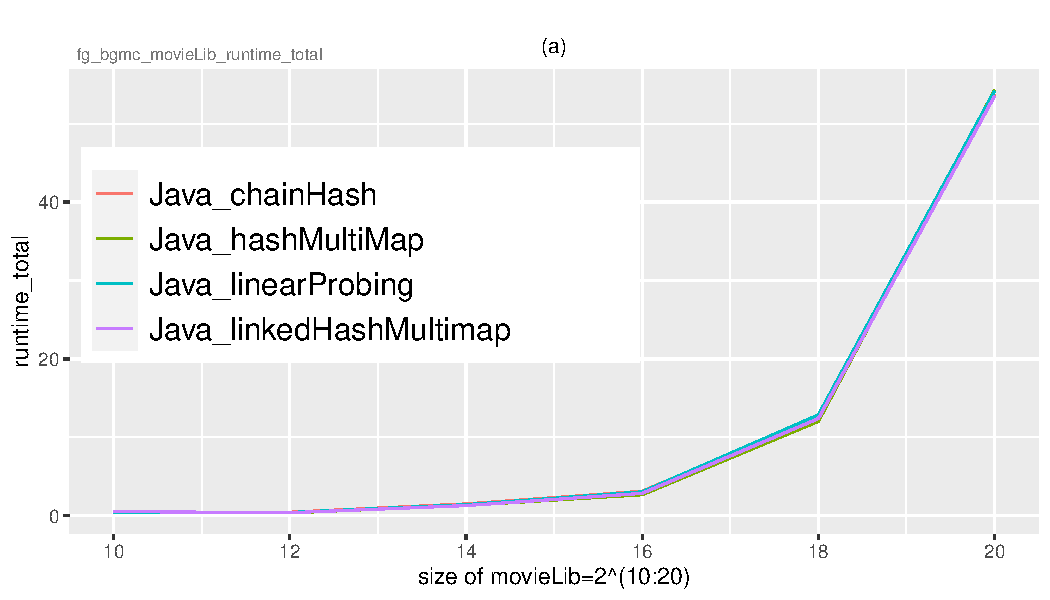
\includegraphics[width=0.45\textwidth]{../_Figures/fg_bgmc/fg_bgmc_movieLib_runtime_total_a}
%\end{tabular}
%
%&
%
%\begin{tabular}{c} 
%\hspace*{-6ex}
%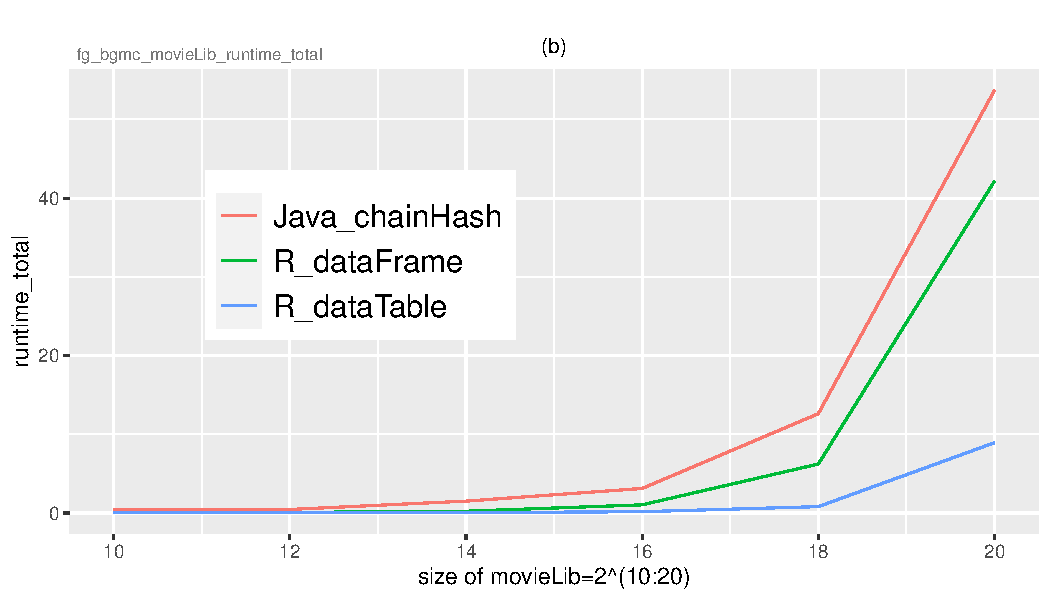
\includegraphics[width=0.45\textwidth]{../_Figures/fg_bgmc/fg_bgmc_movieLib_runtime_total_b}
%\end{tabular}
%
%\\[1ex]
%
%\begin{tabular}{c} 
%\hspace*{-6ex}
%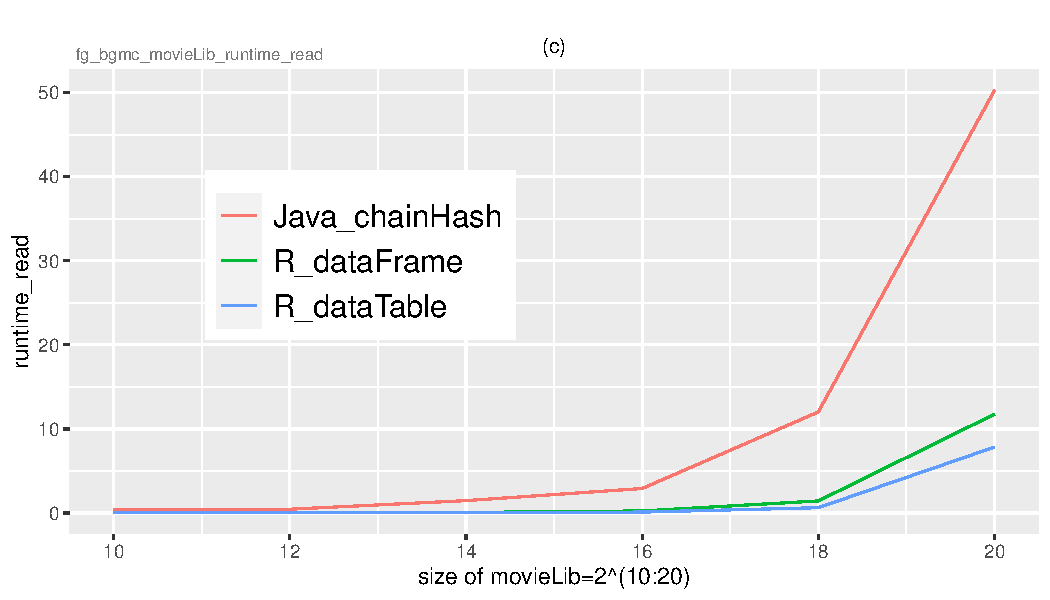
\includegraphics[width=0.45\textwidth]{../_Figures/fg_bgmc/fg_bgmc_movieLib_runtime_read_c}
%\end{tabular}
%
%&
%
%\begin{tabular}{c} 
%\hspace*{-6ex}
%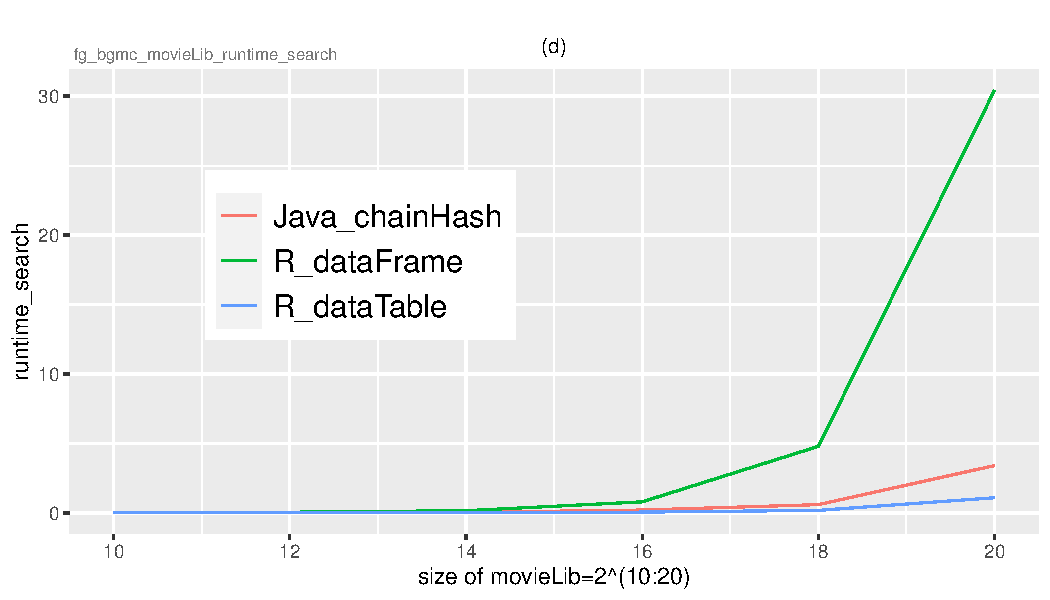
\includegraphics[width=0.45\textwidth]{../_Figures/fg_bgmc/fg_bgmc_movieLib_runtime_search_d}
%\end{tabular}
%
%\end{tabular} 

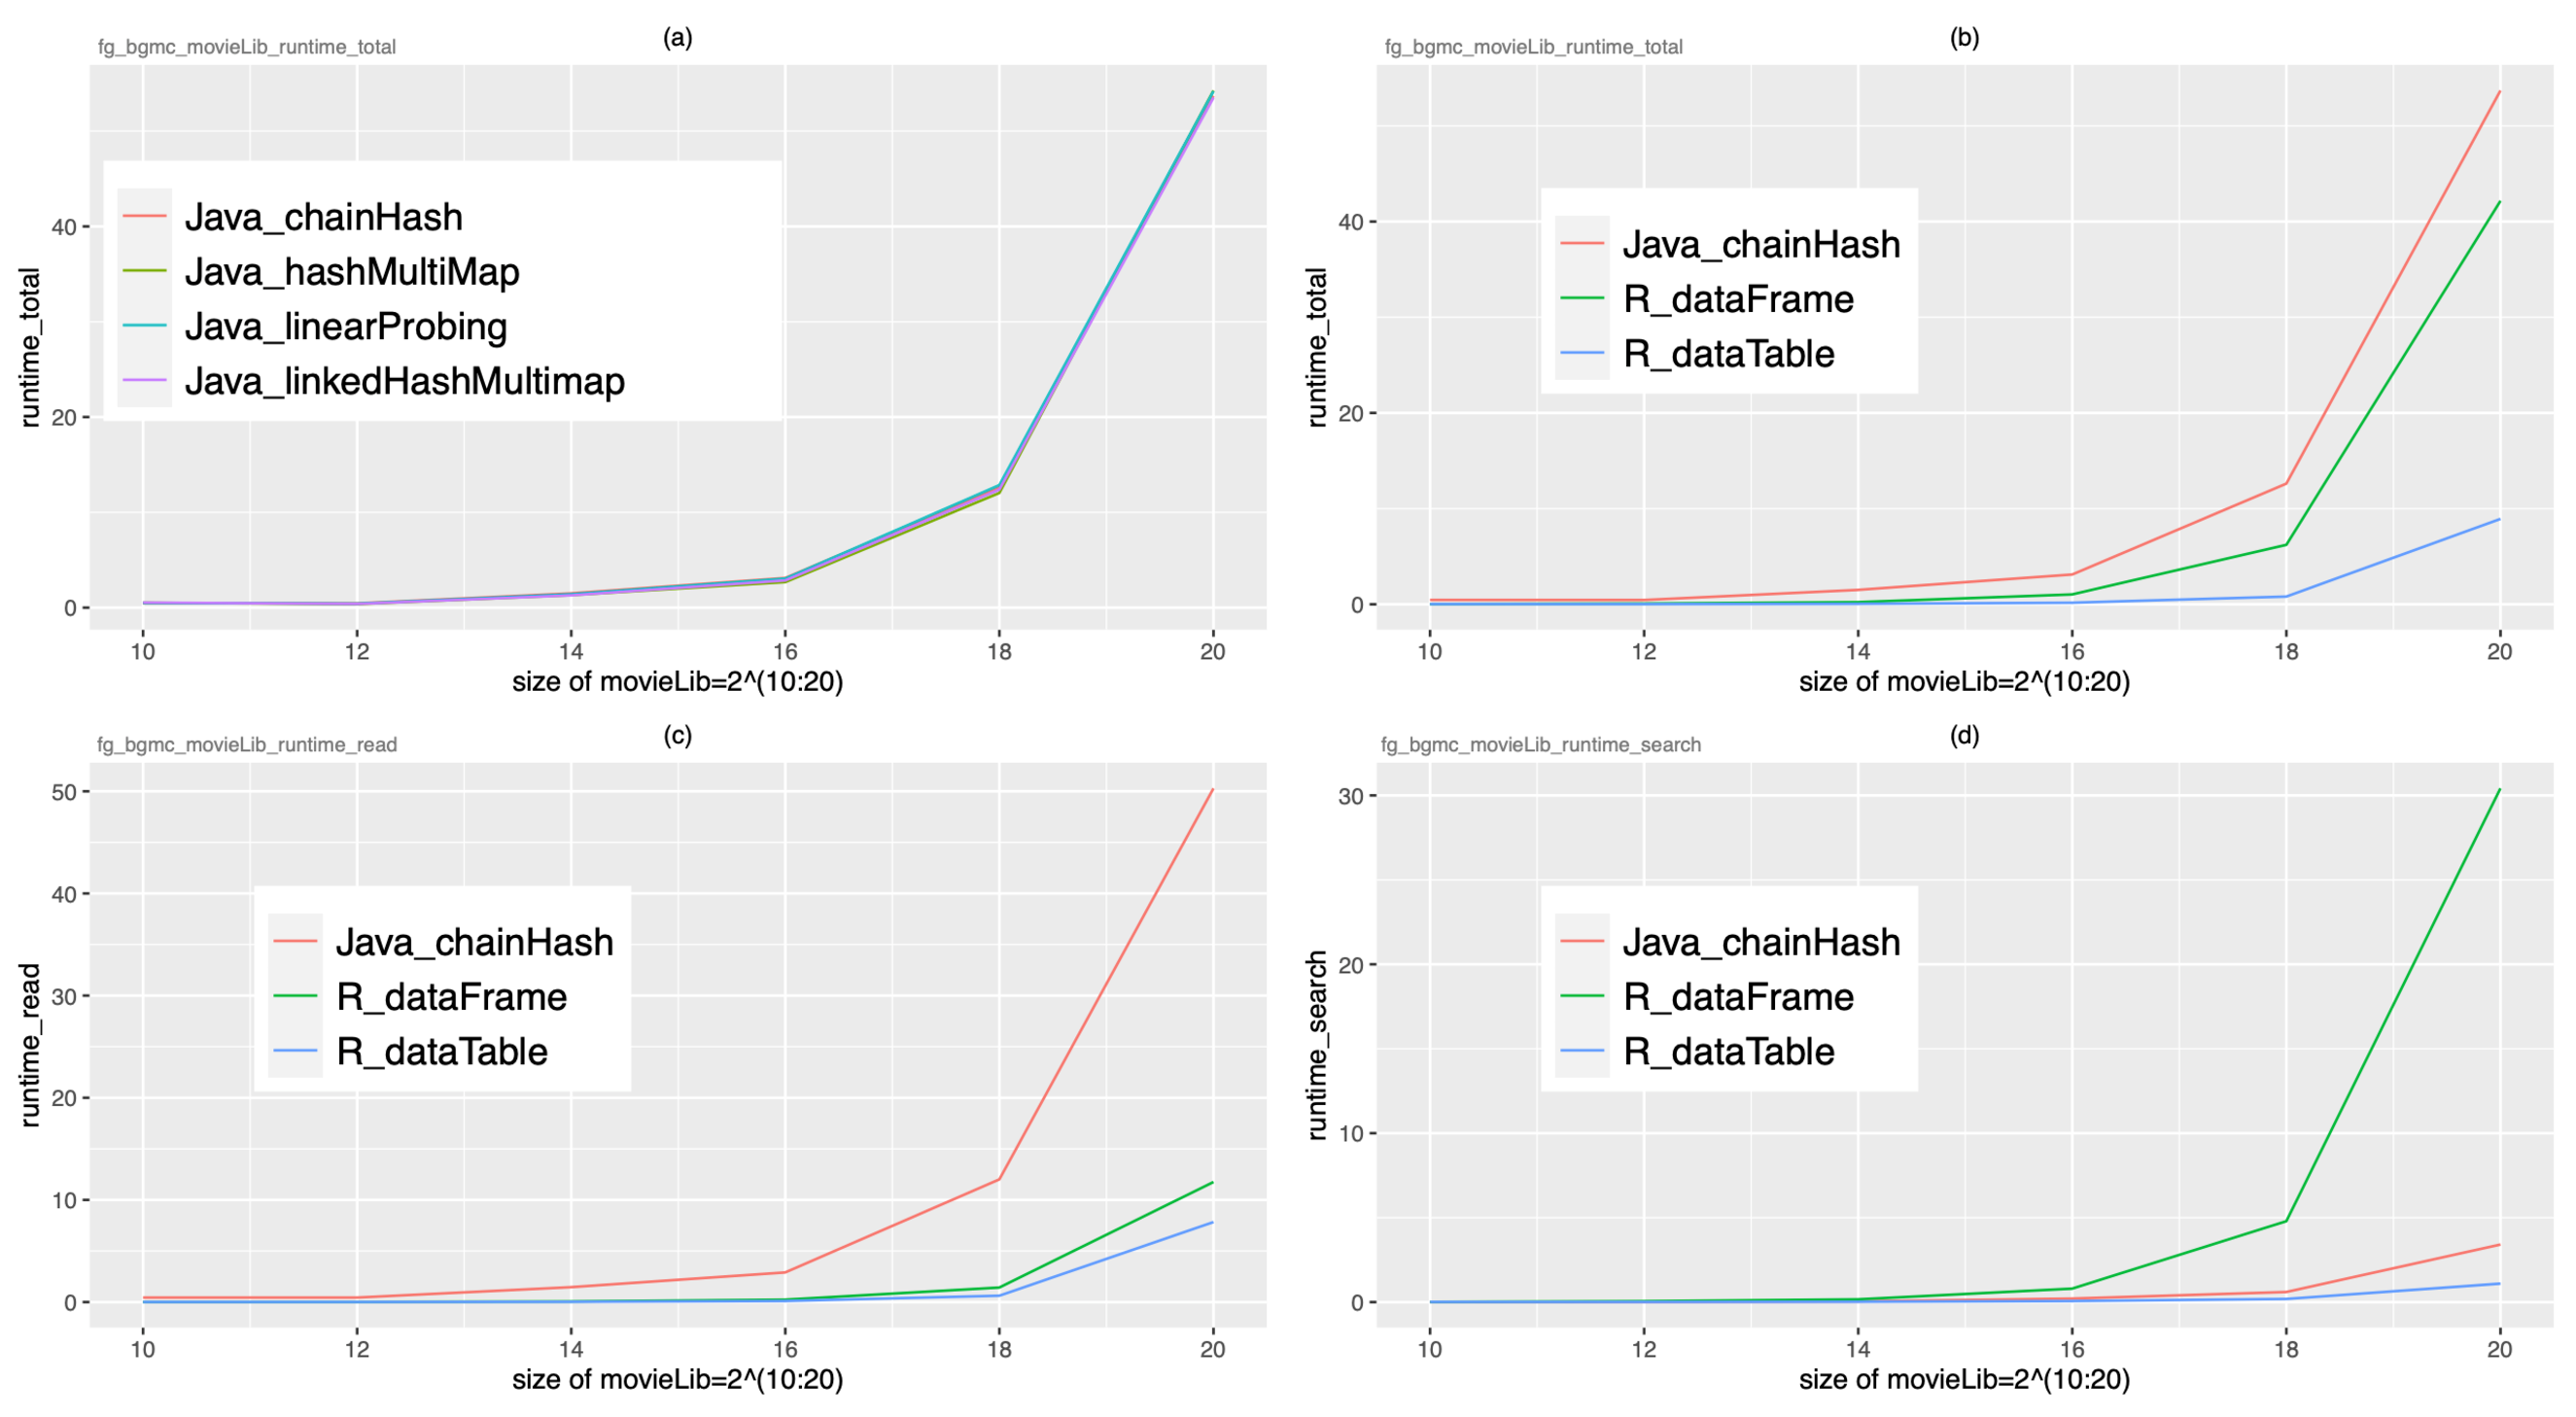
\includegraphics[width=1.0\textwidth]{_Figures/fg_bgmc_movieLib_runtime_abcd}

\caption{
Asymptotic runtime performance experiments with instances from {\it movieLib}, 
based on Java and R code. In each case, the objective is to retrieve the top 10
movies after reading two sets of files: one listing movies and one listing 
viewer interactions with each movie.
In (a), we report {\it runtime\_total} for best four data structures in Java; 
a model used in CSC316 class.
In (b), we report on {\it runtime\_total} for the single best data structure in Java ({\t chainHash}) in comparison with two best data structures in R ({\t dataFrame} and {\t dataTable}).
In (c), we report {\it runtime\_read} for {\it chainHash} in Java and {\it dataFrame} and {\it dataTable}
in R.
In (d), we report {\it runtime\_search} for {\it chainHash} in Java and {\it dataFrame} and {\it dataTable}
in R.
There is no doubt that, for  instances from {\it movieLib}, 
R significantly outperforms Java -- with {\it dataTable} an asymptotically better data structure in 
comparison with {\it dataFrame}.
}
\OMIT{
\caption{Experiments that analyze the total runtime, reading runtime and searching runtime for all Java and R programs. Data table version in R has a significantly improvement in runtime performance comparing to the others. The main obstacle that slows down the Java program is when reading data files and converting each line of information into an object. However, the Java program runs relatively fast when manipulating in the movieLib. Overall, the data table version of R program outperforms in any aspect including reading files and searching movies.}
}
\label{fg_bgmc_movieLib_runtime}
\end{figure*}


\subsection{{\sf Data Structures and Java Libraries}}
\noindent
Data structures introduced in CSC316 are standard Java libraries introducing a number of Java ADTs, from {\it Linked List} to {\it Linear Probing Hash Map}.

\par\vspace*{0.9ex}
In this article, we extend our runtime performance experiments to additional Java ADTs:
{\it Hash MultiMap} and {\it Linked Hash MultiMap} from
{\it Google Guava}~\cite{OPUS-csc316-guava} and  {\it Chain Hash Map} from
{\it net.datastructures}, posted at the Brown University~\cite{OPUS-csc316-net-datastructure}.

\par\vspace*{0.9ex}
The Java code uses Map ADT to pair each key and value.
Initially, our R code also paired each key with a value using a hash function. 
However, the runtime performance was worse than Java ADT.
This led to exploration of two data structures in R:
{\tt data.frame}~\cite{OPUS-csc316-data-frame} and 
{\tt data.table}~\cite{OPUS-csc316-data-table}. 
The {\it Eureka moment} came with the observation that  
{\tt data.table} in R significantly
outperforms the best Java version. For details,
see Figure~\ref{fg_bgmc_movieLib_runtime}.
\par\vspace*{0.9ex}

\subsection{{\it \sf Runtime experiments: Java vs R}}
\noindent
%
The four plots in Figure~\ref{fg_bgmc_movieLib_runtime},
illustrate the runtime performance for {\tt PackFlix} in Java and R. 
In the previous section, we introduced four Map ADTs in Java, 
which are from course work and public domain. 

\begin{description}

\item[\sf{Plot in Figure~\ref{fg_bgmc_movieLib_runtime}a}]~\\\
is a repeat of  experiments in CSC316:
it depicts {\tt runtime\_total} of {\tt PackFlix} with the Map ADTs from Java. 
Results show that these runtimes are statistically equivalent. 
For the follow-up experiments in
Figures~\ref{fg_bgmc_movieLib_runtime}b,c,d
we select 
{\tt Java\_chainHash} as a representative of the best Java ADTs to be compared with the two  ADTs in R.


\item[\sf{Plot in Figure~\ref{fg_bgmc_movieLib_runtime}b}]~\\\
depicts {\tt runtime\_total} of {\tt PackFlix} with 
{\tt Java\_chainHash},
{\tt R\_dataFrame}, and 
{\tt R\_dataTable}. 
Here, we observe that {\tt runtime\_read} of {\tt PackFlix} under Java is 
significantly outperformed by {\it both} ADTs in R.
Questions that arise are these:\\
(1) Which ADT is the best when reading files and initializing the respective data structures?\\
(2) Which ADT is the best when searching the dataset before returning the top 10 movies?
%Why is R program in data table way faster than the other two? Or what is the main 
%obstacle to slow down the runtime for the rest two programs. To answer the questions, 
%we separate the total runtime performance into runtime for reading files and runtime 
%for searching the dataset. 

\item[\sf{Plot in Figure~\ref{fg_bgmc_movieLib_runtime}c}]~\\\
depicts only the {\tt runtime\_read} of {\tt PackFlix} with 
{\tt Java\_chainHash},
{\tt R\_dataFrame}, and 
{\tt R\_dataTable}. 
Again, we observe that {\tt runtime\_read} of {\tt PackFlix} under Java is 
significantly outperformed by {\it both} ADTs in R.
In principle, Java can read large datasets efficiently. 
However, in {\tt PackFlix}, it not only needs to read line by line from each data files, 
but it also needs to convert each line of data into objects and save them into a global array. This appears as the major factor that Java programs in {\tt PackFlix} cannot compete with ADTs in R. 
This question best left to R developers:
why does {\tt R\_dataTable}, under  {\tt runtime\_read},
start to outperform {\tt R\_dataFrame} at 
instance sizes $\ge 2^{18}$?
%However, the runtime for reading files in the other R program with data frame is similar to the R program with data table. Then, a followup question arises: why is data frame slow?

\item[\sf{Plot in Figure~\ref{fg_bgmc_movieLib_runtime}d}]~\\\
focuses on the {\tt runtime\_search} of {\tt PackFlix} with 
{\tt Java\_chainHash},
{\tt R\_dataFrame}, and 
{\tt R\_dataTable}. 
All of these programs return the same list of 
{\it the top 10 most frequently watched movies}.
However, there are significant differences 
in the {\tt runtime\_search} %before returning this list
for the largest movie list with $2^{20}$ titles.
Again, {\tt R\_dataTable} significantly outperforms
{\tt Java\_chainHash}. But here, {\tt Java\_chainHash}
significantly outperforms {\tt R\_dataFrame}.
Another question for developers of R:
why does the gap in {\tt runtime\_search} between {\tt R\_dataFrame}
and {\tt R\_dataTable} increases so rapidly 
for {\em this dataset}?

%In plot (d), we test the runtime for searching most popular movies. The surprising point is that Java program has an excellent performance when searching the data, but the data frame version cannot fast retrieve the most popular movies. The reason why R program with data table is fast is because data table library has C program as the backup engine. Data table library produces efficient runtime performance when reading files and manipulating datasets.

\end{description}

\subsection{Correlation Experiments with {\tt MovieLib} Dataset}
\noindent
%
We complete the analysis of experiments with {\tt PackFlix} and 
the {\tt MovieLib} dataset by a frequency analysis of the 
top 10 movie watched and the total number of movies watched 
for the largest movie list with $2^{20}$ titles.

\begin{description}

\item[\sf{Plot in Figure~\ref{fg_bgmc_movieLib_best10}a}]~\\\
depicts the frequency of top 10 movies watched. % For example, 
The movie with index 1 has been watched 9 times, movies with indices 2-9 have been watched 8 times, etc.
%{\bf Eason, pls fix y-axis to list (0,2,4,6,8,10)}


\item[\sf{Plot in Figure~\ref{fg_bgmc_movieLib_best10}b}]~\\\
counts the total number of movies watched: %For example, 
385,128 movies have been watched only once (index = 1), 75 movies have been watched 7 times (index = 7), only one movie has been watched 9 times (index = 9).

\end{description}
%
%
%is a repeat of  experiments in CSC316:
%it depicts {\tt runtime\_total} of {\tt PackFlix} with the Map ADTs from Java. 
%Results show that these runtimes are statistically equivalent. 
%For the follow-up experiments in
%Figures~\ref{fg_bgmc_movieLib_runtime}b,c,d
%we select 
%{\tt Java\_chainHash} as a representative of the best Java ADTs to be compared with the two  ADTs in R.
%
%using the dataset of size $2^{20}$. 
%After testing the runtime performance for Java and R programs, we want to fully analyze the {\tt PackFlix}. Then, in Figure~\ref{fg_bgmc_movieLib_best10}, 
%we generate two plots that depict the frequency of 
% 
%
%\TOPIC{movieLib: best ten}
%In plot (a) of Figure~\ref{fg_bgmc_movieLib_best10}, it 
%\TOPIC{movieLib: best ten occurences}
%The plot (b) of of Figure~\ref{fg_bgmc_movieLib_best10} counts the total number of movies watched. For example, 385128 movies have been watched only once (index = 1), 75 movies have been watched 7 time (index = 7), only one movie has been watched 9 times (index = 9).

\begin{figure}[h!]
\vspace*{-2ex}
\centering
%\setlength{\tabcolsep}{3pt} % Default value: 6pt
%\renewcommand{\arraystretch}{0.5} % Default value: 1


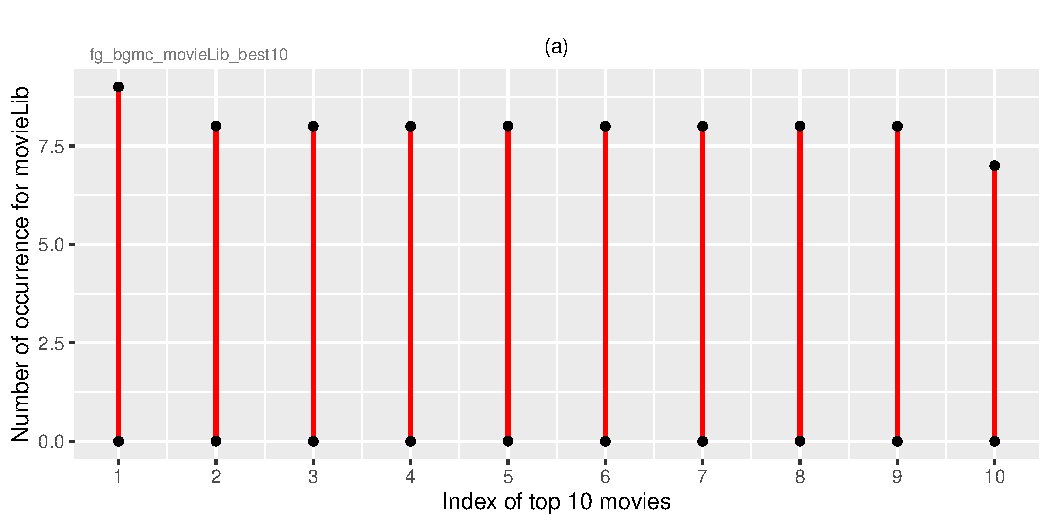
\includegraphics[width=0.48\textwidth]{_Figures/fg_bgmc_movieLib_best10}
\\[2ex]
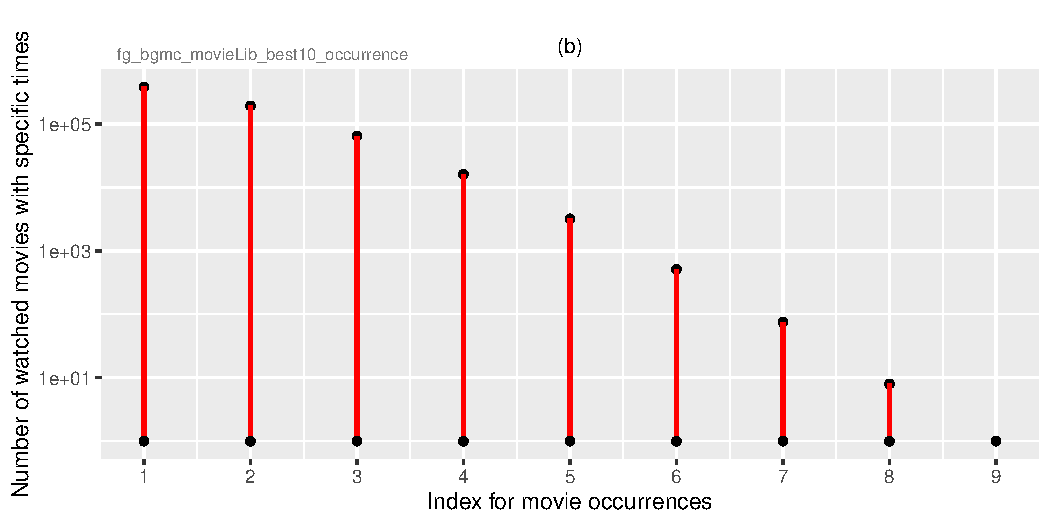
\includegraphics[width=0.48\textwidth]{_Figures/fg_bgmc_movieLib_best10_occurrence}


\caption{
These two plots relate results for the largest movie list with $2^{20}$ titles.
The plot (a) depicts the frequency of top 10 movies watched. For example, the movie with index 1 has been watched 9 times, movies with indices 2-9 have been watched 8 times, etc. 
\\
The plot (b) counts the total number of movies watched. For example, 385128 movies have been watched only once (index = 1), 75 movies have been watched 7 times (index = 7), only one movie has been watched 9 times (index = 9).
\vspace*{-3ex}
}
\label{fg_bgmc_movieLib_best10}
\end{figure}


%\subsection{Lessons learned ...}
%\noindent
%%
%In this section, we described what the {\tt PackFlix} is and how it related to this paper. Then, we tested our programs with asymptotic experiments to find the runtime performance based on different data structures. It is a good start for illustrating the concepts of this paper, which includes introducing the bipartite graphs, the relationship between runtime performance with data structures, and the importance of using asymptotic experiments to generate precise and accurate results.








